\section{Assess ecological status from 1990-2020}

\begin{frame}{Assess ecological status from 1990-2020}
  Construct a complete panel dataset of ecological status for 1990-2020 comprising every Danish waterbody\pause:
  \begin{enumerate}
    \item Biologists' field observations with GPS coordinates.
    \pause
    \item Assign point observations to matching water bodies.
    \pause
    \item Impute missing observations.
    % \begin{itemize}
    %   \item Estimated by \textit{multivariate imputation by chained equations (MICE)} where a \textit{fully conditional specification (FCS)} is constituted by a conditional density for each year.
    %   \item Physical characteristics are included in a \textit{Bayesian ridge regression} using \textit{iteratively-reweighted regularized least-squares}.
    % \end{itemize}
    % \item Extrapolation of ecological status of streams for 1990 and 1991.
    \pause
    \item Translate biological indicators into ecological status being “Bad”, “Poor”, “Moderate”, “Good”, or “High”.
  \end{enumerate}
  \note<1>{\textit{This project consists of three parts.}\\\bigskip
    \textbf{\nth{1} part} is to \textbf{(...)} i.e. for all streams, lakes, fjords, coastal waters and groundwater bodies. Process:
  }
  \note<2>{\begin{enumerate}
    \item ... In the case of several observations in a year: apply the EU WFD's conservative approach of using the observation indicating the worst quality.
  \end{enumerate}
  }
  \note<3>{\begin{enumerate}
    \item 
    \item ... included in the current Danish waterbody plan (VP2).
  \end{enumerate}
  }
  \note<4>{\begin{enumerate}
    \item 
    \item 
    \item ... on the basis of observations of other waterbodies for the given year as well as observations from other years and a few physical characteristics. Issue: data isn't representative but has a systematic overrepresentation of larger waterbodies and those of special concern for the ecological quality.
    % \item ... by estimating a linear trend and using it to predict.
  \end{enumerate}
  }
  \note<5>{\begin{enumerate}
    \item 
    \item 
    \item 
    \item ... based on certain thresholds given by the WFD.
  \end{enumerate}
  }
\end{frame}

\begin{frame}{Missing observations for streams}
  \center
  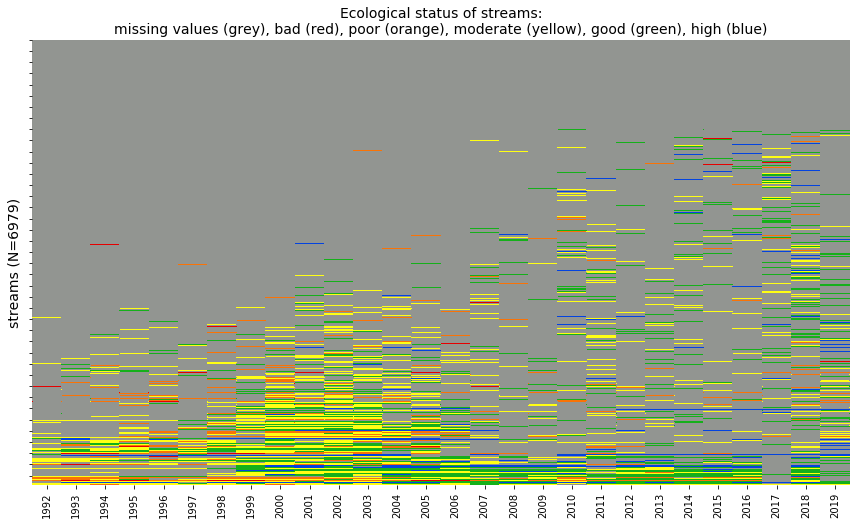
\includegraphics[width=\textwidth]{C:/Users/au687527/GitHub/GNNP/gis/output/missing_streams}
  \note{Heat map for each of the 7000 streams in VP2.\\\bigskip
  Grey indicates missing observations while a different color indicates the observed ecological status in a given year, i.e.
  \begin{itemize}
    \item Top: 9 \% of streams that has never been observed but still has a goal of achieving 'good' ecological status in VP2.
    \item Bottom: Streams observed most years.
    \item Throughout the 90s, $\frac{2}{3}$ of observations were poor/moderate.
    \item From 2009, majority of observations were good/high quality.
    \begin{itemize}
      \item Action Plan on the Aquatic Environment I (1987)
      \item Action Plan on the Aquatic Environment II (1998)
      \item Water Plan I (adopted by parliament 2009, municipal action plans 2010, measures came into effect 2012)
    \end{itemize}
  \end{itemize}
  }
\end{frame}

\begin{frame}
  \center
  \vspace{-1.4cm}
  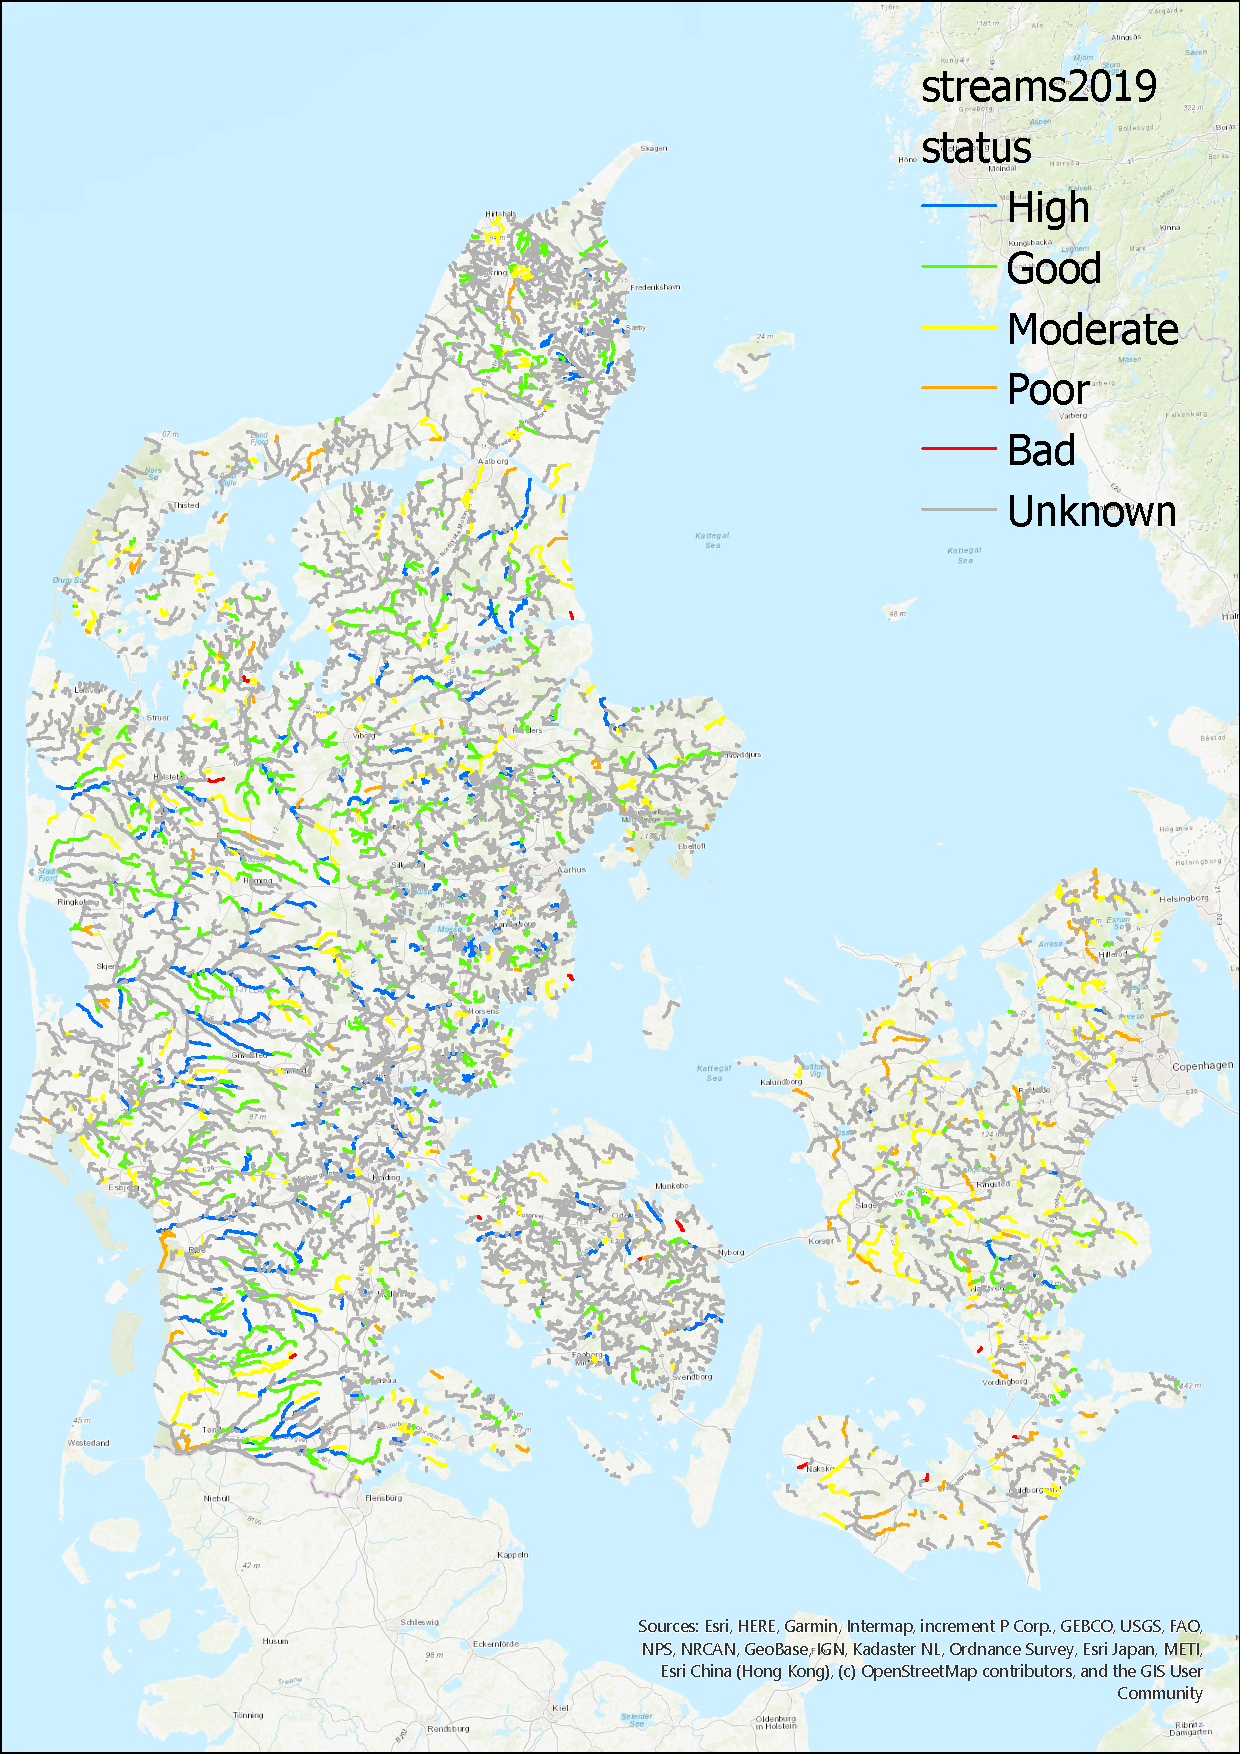
\includegraphics[width=.7\textwidth]{C:/Users/au687527/GitHub/GNNP/gis/output/streams2019}
  \note{In 2019, water quality is still mostly poor/moderate in Eastern DK.
  \\\bigskip
  On average, a quarter of the total stream length is assessed each year; grey lines represent unobserved streams.
  }
\end{frame}